\chapter{CSR-Based Multi-Retailer Reverse-Logistics Network with Shapley Cost Sharing: A U.S. EV Battery Recycling Case}
\label{chap:model2}

Chapter~\ref{chap:model1} studied CSR as a bilateral governance problem. A single Manufacturer and a single Retailer chose prices and CSR-driven recycling maturity, and the analysis showed that the party that creates CSR value, the party that pays for CSR effort, and the party that captures the resulting profit need not be the same. That insight raises a question the bilateral model cannot answer. When CSR responsibility is spread across a manufacturer and many downstream retailers, the strategic object is no longer the maturity level of one retailer-facing program. It is the design and financing of a shared CSR infrastructure: which facilities to open, which processors to contract, how much of the return stream is credibly captured, and---most contentiously---who pays for what. This chapter develops Study~2 of the dissertation around that question.

The theoretical focus of the chapter is therefore CSR governance, and EV battery recycling is the application that makes the governance problem concrete. End-of-life batteries involve safety, environmental, regulatory, and critical-mineral concerns. In the United States, EPA guidance states that lithium-ion batteries should not be placed in household garbage or municipal recycling bins, and that medium- and large-scale batteries, including automobile batteries, should be managed through manufacturers, dealers, installers, or other specialized channels \cite{EPA2026UsedLithiumIon}. For businesses, discarded lithium-ion batteries may be hazardous waste under RCRA, and EPA recommends that many business generators manage them under universal-waste regulations while also noting continuing rulemaking for lithium batteries \cite{EPA2026UniversalWaste}. These conditions create exactly the tension the chapter studies: the Manufacturer faces brand and compliance responsibility for the end-of-life system, while geographically dispersed retailers control the practical collection interface. Neither side can implement credible CSR alone, and neither side will finance a shared system it perceives as unfair.

The chapter asks three research questions. First, how should a CSR-driven reverse-logistics network be designed when collection responsibility is distributed across multiple independent retailers with different volumes, locations, and capabilities? Second, once the efficient shared network is known, how should its net compliance and recovery cost be allocated between the Manufacturer and the retailers? Third, under what conditions does a Shapley-based allocation actually sustain participation and coalition stability, and what governance instruments are available when it does not?

To answer these questions, the chapter develops one integrated model with two analytical phases. Phase~I formulates a mixed-integer linear program (MILP) that computes, for every possible coalition of players, the least-cost CSR-compliant reverse-logistics network and its \emph{net CSR stewardship cost}. Phase~II treats those optimized coalition costs as the characteristic function of a cooperative cost game and studies Shapley allocation, participation, and core stability.

Three features distinguish this design from the existing literature. First, the characteristic cost function of the cooperative game is \emph{derived} from the physical network-design problem rather than assumed: the game allocates a cost that a real coalition would actually incur, facility openings and processor contracts included. Second, CSR capability enters the model as a multi-dimensional primitive---traceability, due diligence, and collaborative governance---that changes feasibility and cost \emph{before} optimization, rather than as a scalar effort or preference weight appended to a profit function. Third, allocation stability is treated as a governance diagnostic rather than a mathematical afterthought: when the Shapley value fails a participation or core check, the chapter provides explicit remedies in the form of hybrid responsibility rules, constrained projections, least-core relaxation, and Manufacturer support, each with a precise economic role.

The remainder of the chapter is organized as follows. Section~\ref{sec:ch4_literature_gap} positions the model within the CSR, reverse-logistics, and cooperative-game literatures. Section~\ref{sec:problem_desc} describes the CSR network architecture and states the modeling assumptions and notation. Section~\ref{sec:milp} develops the coalition-dependent MILP and its analytical properties. Section~\ref{sec:game_theory} defines the cooperative cost game, the Shapley allocation, and the stability diagnostics and remedies. Section~\ref{sec:properties} establishes the main allocation-level results. Section~\ref{sec:case_study} applies the framework to a stylized U.S. EV battery recycling case. Section~\ref{sec:ch4_discussion} draws together the governance insights, the novelty of the framework, its limitations, and the research directions it opens. Section~\ref{sec:model_conclusion} concludes. Detailed proofs are collected in Appendix~\ref{app:ch4_proofs}.

% ============================================================
\section{Literature-Based Research Gap}
\label{sec:ch4_literature_gap}
% ============================================================

The literature review identifies a CSR design problem that is broader than any single recycling technology. CSR is increasingly modeled as a strategic object inside supply chains rather than as a peripheral ethical statement. Game-theoretic CSR studies show that social responsibility can affect commitment, price competition, transparency, retailer effort, channel profitability, and cooperation incentives \cite{Buccella2024,FantiBuccella2017,Ferrara2017,Khosroshahi2019,Mahdiraji2023}. In closed-loop and recycling-oriented settings, CSR and fairness concerns further alter coordination outcomes and cooperation-mode choices \cite{ZhangLiang2023,ZhengB2022}. These studies motivate the chapter's basic premise: CSR becomes economically meaningful only when it is translated into operating responsibilities, cost burdens, and governance rules among independent firms.

A limitation of much CSR supply-chain research is that the physical design of CSR implementation is often abstracted away. Prior models frequently represent CSR as an effort level, preference weight, transparency variable, or investment parameter. That abstraction is useful for deriving strategic incentives, but it does not show how a CSR commitment is implemented when responsibility is distributed across a manufacturer and multiple downstream retailers. A multi-retailer reverse-logistics system makes this issue explicit. Retailers provide local collection access and customer-facing credibility, while the Manufacturer may provide compliance infrastructure, processor contracts, traceability standards, and brand-level CSR accountability. The resulting question is not only whether firms prefer CSR, but how the CSR infrastructure should be designed and how its cost should be governed.

EV battery recycling is used in this chapter as an applied setting that makes this CSR design problem observable. The reverse-logistics literature shows that end-of-life battery systems require facility-location decisions, collection flows, consolidation, processing capacity, and recovery-value management \cite{tadaros2022location,bafadal2024proposed,wang2025planning,ma2024unlocking}. These studies establish the operational importance of network design. However, when they optimize flows and facilities, they often treat the system as if a central planner can finance and implement the network. From a CSR governance perspective, that is incomplete: the optimized network cost must still be assigned to independent stakeholders whose incentives and responsibilities are not identical.

The cooperative-game literature provides the fairness and stability language needed for this second problem. Shapley allocation and related solution concepts have been used to study horizontal logistics cooperation, collaborative distribution, multi-echelon supply-chain allocation, and operations-management cost or profit sharing \cite{lozano2013cooperative,wang2023collaborative,meng2023profit,luo2022core}. Recent closed-loop and EV battery recycling studies also show that alliance design, cost sharing, and cooperative recycling mechanisms can change system outcomes \cite{ZhengB2022,Xiao2024}. Yet these allocation models often begin from an externally specified cost or surplus. They do not always derive the characteristic cost function from the same physical CSR network that the firms must operate.

This chapter addresses the gap by linking CSR design and CSR cost governance in one framework. The MILP module designs the shared reverse-logistics infrastructure and computes the coalition-dependent net CSR compliance cost. The cooperative-game module then uses that optimized cost as the characteristic function for Shapley allocation. The contribution is therefore not only a network model and not only a cost-sharing rule. It is an integrated CSR governance model that connects operational feasibility, fair cost allocation, individual participation, and coalition stability. Section~\ref{sec:ch4_discussion} returns to this positioning after the analysis, contrasting the framework with effort-scalar CSR models and centrally planned network studies, and mapping its capability constructs onto contemporary CSR governance and due-diligence frameworks.

% ============================================================
\section{Problem Description and Model Assumptions}
\label{sec:problem_desc}
% ============================================================

Consider a Manufacturer, denoted by $M$, and a set of independent retailers, denoted by $I=\{1,\ldots,n\}$. Each retailer $i\in I$ collects a deterministic volume $d_i$ of end-of-life products over a planning horizon. In the U.S. EV battery case, the retailers represent regional dealer or service networks that receive retired batteries from consumers, fleets, service operations, or warranty channels. The Manufacturer carries brand-level and CSR responsibility for the end-of-life system, while retailers provide the local interface through which returns enter the reverse channel.

The reverse network contains three physical echelons:
\begin{enumerate}
    \item \textbf{Retailer collection nodes.} Retailers collect, inspect, package, and prepare returned batteries for shipment.
    \item \textbf{Consolidation centers.} Candidate facilities aggregate returns from multiple retailers, perform sorting and safety handling, and prepare batches for downstream recovery.
    \item \textbf{Recovery or recycling processors.} Candidate processors recover usable materials or provide certified treatment. In the case study, one processor represents a high-fixed-cost, high-recovery technology and another represents a lower-fixed-cost, lower-recovery option.
\end{enumerate}

The CSR interpretation is important. The network is not only a cost-minimizing logistics system. It is an institutional mechanism for making the Manufacturer's CSR promise credible. Retailers generate local collection volume, the Manufacturer can provide compliance infrastructure and processor contracts, and the coalition must decide how to finance a network whose benefits are system-wide.

\begin{figure}[htbp]
\centering
\begin{tikzpicture}[
    node distance=1.7cm and 2.7cm,
    retailer/.style={circle, draw=blue!60, fill=blue!5, very thick, minimum size=1.05cm, align=center},
    center/.style={rectangle, draw=orange!70, fill=orange!8, very thick, minimum width=1.25cm, minimum height=0.9cm, align=center},
    plant/.style={regular polygon, regular polygon sides=6, draw=green!60!black, fill=green!7, very thick, minimum size=1.25cm, align=center},
    csr/.style={rectangle, draw=black!45, fill=black!4, rounded corners=2pt, align=center, font=\small},
    arrow/.style={-{Stealth[scale=1.1]}, thick, draw=gray!80}
]

\node[csr] (m) {Manufacturer\\CSR platform};

\node[retailer] (r1) [below left=0.3cm and 2.4cm of m] {$R_1$};
\node[retailer] (r2) [below=of r1] {$R_2$};
\node[retailer] (r3) [below=of r2] {$R_3$};

\node[center] (c1) [right=of r1, yshift=-0.8cm] {$C_1$};
\node[center] (c2) [right=of r2, yshift=-0.8cm] {$C_2$};

\node[plant] (p1) [right=of c1, yshift=-0.8cm] {$P_1$};
\node[plant] (p2) [right=of c2, yshift=-0.8cm] {$P_2$};

\draw[arrow] (m) -- (c1);
\draw[arrow] (m) -- (c2);

\draw[arrow] (r1) -- (c1) node[midway, above, sloped, font=\scriptsize] {$q_{11}$};
\draw[arrow] (r1) -- (c2);
\draw[arrow] (r2) -- (c1);
\draw[arrow] (r2) -- (c2) node[midway, above, sloped, font=\scriptsize] {$q_{22}$};
\draw[arrow] (r3) -- (c1);
\draw[arrow] (r3) -- (c2);

\draw[arrow] (c1) -- (p1) node[midway, above, sloped, font=\scriptsize] {$x_{11}$};
\draw[arrow] (c1) -- (p2);
\draw[arrow] (c2) -- (p1);
\draw[arrow] (c2) -- (p2) node[midway, below, sloped, font=\scriptsize] {$x_{22}$};

\node[above=0.25cm of r1, font=\bfseries] {Retail collection};
\node[above=0.85cm of c1, font=\bfseries] {Consolidation};
\node[above=0.85cm of p1, font=\bfseries] {Recovery};

\end{tikzpicture}
\caption{CSR-Based Multi-Retailer Reverse-Logistics Network}
\label{fig:network_structure}
\end{figure}

Figure~\ref{fig:network_structure} summarizes the logic. Physical flows move from retailers to consolidation centers and then to processors. CSR support moves in the other direction: the Manufacturer can provide platform investment, compliance routines, processor contracts, traceability systems, and recovery-value access that reduce the coalition's net compliance cost.

\subsection{Model Assumptions and Notation}
\label{sec:notation}

The baseline model rests on six assumptions, stated here in the order in which they enter the analysis.

The first two assumptions fix the institutional setting. The reverse-logistics system is interpreted as a CSR responsibility shared by the Manufacturer and the participating retailers: retailers supply local collection volume, while the Manufacturer can provide system-level compliance support, processor access, and recovery contracts. Each retailer's end-of-life return volume $d_i$ is treated as known for the planning horizon. This deterministic-volume assumption represents expected annual returns and provides a stable baseline for strategic network design; Section~\ref{sec:ch4_discussion} discusses its relaxation.

The third assumption concerns formal-channel responsibility. The CSR system aims to route end-of-life returns through formal, certified recovery or treatment channels. Because traceability is imperfect in many distributed collection systems, the model permits an analytically defined leakage variable. Leakage does not represent an acceptable disposal choice; it represents unaccounted or informally managed returns that create CSR risk and penalty cost. Modeling leakage explicitly, rather than assuming it away, is what allows the analysis to separate the operational cost of collection from the governance cost of proving that collection actually happened.

The fourth assumption gives the model its cost structure. Transportation, handling, processing, and recovery values are linear in shipped volume, while opening consolidation centers and processors involves fixed costs. This combination of linear variable costs and binary facility decisions is what makes coalition costs nonlinear in membership and, as shown later, is the source of both cooperation gains and potential instability.

The remaining two assumptions are load-bearing for the cooperative analysis in Phase~II. \emph{Transferable cost:} coalition members can make monetary transfers after the network cost is computed, so that the Shapley value can allocate the coalition's optimized net CSR compliance cost. \emph{Coalition-dependent CSR capability:} for each coalition $S$, the level of CSR implementation capability is represented by parameters that are fixed before the network problem is solved. The optimization model therefore remains a MILP for each coalition, while comparative statics can evaluate how better governance capability changes the optimized cost.

The notation is summarized in Table~\ref{tab:ch4-notation}. A coalition is denoted by $S\subseteq N$, where $N=\{M\}\cup I$. The participating retailers in coalition $S$ are $I(S)=S\cap I$.

\begin{table}[htbp]
\centering
\caption{Sets, Parameters, and Decision Variables for Chapter 4}
\label{tab:ch4-notation}
\resizebox{\textwidth}{!}{%
\begin{tabular}{ll}
\toprule
\textbf{Symbol} & \textbf{Description} \\
\midrule
$I$ & Set of retailers, indexed by $i$ \\
$J$ & Set of candidate consolidation centers, indexed by $j$ \\
$L$ & Set of candidate recovery processors, indexed by $l$ \\
$N$ & Set of cooperative-game players, $N=\{M\}\cup I$ \\
$S$ & Coalition of players, $S\subseteq N$ \\
$I(S)$ & Retailers participating in coalition $S$, $I(S)=S\cap I$ \\
\midrule
$d_i$ & End-of-life return volume collected by retailer $i$ \\
$c_i^R$ & Unit collection and initial CSR handling cost at retailer $i$ \\
$t_{ij}$ & Unit transportation cost from retailer $i$ to consolidation center $j$ \\
$u_{jl}$ & Unit transportation cost from consolidation center $j$ to processor $l$ \\
$f_j^C$ & Fixed cost of opening consolidation center $j$ \\
$h_j$ & Unit handling and sorting cost at consolidation center $j$ \\
$K_j^C$ & Capacity of consolidation center $j$ \\
$f_l^P(S)$ & Coalition-dependent fixed access cost for processor $l$ \\
$p_l(S)$ & Coalition-dependent unit processing/compliance cost at processor $l$ \\
$K_l^P$ & Capacity of processor $l$ \\
$r_l(S)$ & Coalition-dependent recovered-material value per unit at processor $l$ \\
$\rho_l$ & Recovery efficiency factor at processor $l$, $0<\rho_l\leq 1$ \\
$\tau(S)$ & Traceability and transparency capability of coalition $S$, $0\leq \tau(S)\leq 1$ \\
$\eta(S)$ & Due-diligence and compliance maturity of coalition $S$, $0\leq \eta(S)\leq 1$ \\
$\kappa(S)$ & Collaborative governance quality of coalition $S$, $0\leq \kappa(S)\leq 1$ \\
$G(S)$ & Coalition CSR capability vector, $G(S)=(\tau(S),\eta(S),\kappa(S))$ \\
$A_l(S)$ & Eligibility indicator equal to 1 if coalition $S$ can use processor $l$ \\
$\eta_l^{\min}$ & Minimum due-diligence maturity required to contract with processor $l$ \\
$\lambda$ & CSR pressure or compliance-risk weight \\
$\mu_i$ & Penalty cost per unit of unaccounted return from retailer $i$ \\
$g(S;G)$ & Fixed CSR platform, reporting, traceability, and compliance cost borne by coalition $S$ \\
$p_x$ & Baseline CSR responsibility share of player $x$ for hybrid allocation \\
$\theta$ & Weight placed on Shapley allocation in a hybrid allocation rule \\
\midrule
$q_{ij}$ & Flow from retailer $i$ to consolidation center $j$ \\
$x_{jl}$ & Flow from consolidation center $j$ to processor $l$ \\
$\ell_i$ & Unaccounted or informal-channel return volume associated with retailer $i$ \\
$y_j$ & Binary variable equal to 1 if consolidation center $j$ is opened \\
$z_l$ & Binary variable equal to 1 if processor $l$ is used \\
$c(S;G)$ & Optimized net CSR compliance cost of coalition $S$ under CSR capability $G(S)$ \\
$\phi_x(c)$ & Shapley cost allocation to player $x\in N$ \\
$\sigma(S;\phi)$ & Core slack of coalition $S$ under allocation $\phi$ \\
\bottomrule
\end{tabular}%
}
\end{table}

% ============================================================
\section{Phase I: Coalition-Dependent CSR Network Optimization}
\label{sec:milp}
% ============================================================

The first phase computes the least costly CSR-compliant reverse-logistics network for any coalition $S\subseteq N$. Unlike a standard centralized network model, the objective is not simply logistics cost. It is the \emph{net CSR stewardship cost}: the cost of collection, safe handling, transportation, consolidation, processing, compliance infrastructure, traceability, and residual compliance risk, less the value recovered from processed materials.

The distinction matters for CSR research. In much supply-chain CSR modeling, CSR is represented by a scalar effort, preference weight, or transparency parameter \cite{Buccella2024,FantiBuccella2017,Ferrara2017,Khosroshahi2019,Mahdiraji2023}. That abstraction is useful for strategic games, but it hides the physical implementation problem. In a distributed reverse-logistics network, CSR is implemented through collection points, data records, certified handling, processor eligibility, and cost-bearing rules. The model below translates the CSR governance capability of a coalition into operational decisions and then into the characteristic cost used by the cooperative game.

\subsection{Coalition CSR Capability}

For coalition $S$, define the CSR capability vector
\begin{equation}
\label{eq:ch4_governance_vector}
G(S)=\left(\tau(S),\eta(S),\kappa(S)\right),
\qquad
0\leq \tau(S),\eta(S),\kappa(S)\leq 1.
\end{equation}
The parameter $\tau(S)$ represents traceability and transparency capability. A coalition with higher $\tau(S)$ has better visibility of returned units, stronger chain-of-custody documentation, and lower unaccounted flow. The parameter $\eta(S)$ represents due-diligence and compliance maturity. A coalition with higher $\eta(S)$ can satisfy stricter processor-contract requirements, manage hazardous-material obligations more reliably, and document responsible treatment. The parameter $\kappa(S)$ represents collaborative governance quality. A coalition with higher $\kappa(S)$ has better information sharing, lower coordination friction, and more credible joint reporting.

These parameters are not survey variables in this chapter. They are analytical primitives that allow CSR governance to enter the optimization model. A convenient coalition formation rule is the capped additive form
\begin{equation}
\label{eq:ch4_governance_capability}
g_m(S)=\min\left\{1,\ g_m^0+\alpha_{M}^{m}\mathbf{1}_{\{M\in S\}}
+\sum_{i\in I(S)}\alpha_i^{m}\right\},
\qquad m\in\{\tau,\eta,\kappa\},
\end{equation}
where $g_\tau(S)=\tau(S)$, $g_\eta(S)=\eta(S)$, and $g_\kappa(S)=\kappa(S)$. Equation~\eqref{eq:ch4_governance_capability} captures the idea that retailers contribute local collection knowledge and customer-facing execution, while the Manufacturer can contribute platform-level compliance routines, processor contracts, reporting systems, and brand-level accountability. Other monotone capability functions can be used without changing the logic of the model, provided that $G(S)$ is fixed before the coalition-restricted MILP is solved.

\begin{figure}[htbp]
\centering
\begin{tikzpicture}[
    node distance=1.2cm and 1.7cm,
    box/.style={rectangle, draw=black!55, fill=black!4, rounded corners=2pt, align=center, minimum width=2.35cm, minimum height=0.85cm, font=\small},
    effect/.style={rectangle, draw=blue!55, fill=blue!5, rounded corners=2pt, align=center, minimum width=2.35cm, minimum height=0.85cm, font=\small},
    result/.style={rectangle, draw=green!55!black, fill=green!6, rounded corners=2pt, align=center, minimum width=2.4cm, minimum height=0.85cm, font=\small},
    arrow/.style={-{Stealth[scale=1.05]}, thick, draw=gray!85}
]
\node[box] (tau) {$\tau(S)$\\Traceability};
\node[box, below=of tau] (eta) {$\eta(S)$\\Due diligence};
\node[box, below=of eta] (kap) {$\kappa(S)$\\Collaboration};

\node[effect, right=of tau] (leak) {Lower\\leakage risk};
\node[effect, right=of eta] (access) {Processor\\eligibility};
\node[effect, right=of kap] (friction) {Lower\\coordination cost};

\node[result, right=of access, yshift=1.0cm] (cost) {Net CSR\\stewardship cost};
\node[result, right=of access, yshift=-1.0cm] (stability) {Coalition\\stability};

\draw[arrow] (tau) -- (leak);
\draw[arrow] (eta) -- (access);
\draw[arrow] (kap) -- (friction);
\draw[arrow] (leak) -- (cost);
\draw[arrow] (access) -- (cost);
\draw[arrow] (friction) -- (cost);
\draw[arrow] (cost) -- (stability);
\end{tikzpicture}
\caption{CSR Governance Parameters and Their Operational Effects}
\label{fig:ch4_governance_parameters}
\end{figure}

Figure~\ref{fig:ch4_governance_parameters} shows the modeling logic. Traceability affects how much return volume is captured in the formal channel. Due diligence affects whether the coalition can use higher-standard processors and whether compliance costs are reduced. Collaboration affects the fixed and transaction costs of operating the coalition. These effects enter Phase I as cost and feasibility terms; they enter Phase II indirectly through the coalition cost function $c(S;G)$.

\subsection{The Coalition-Dependent MILP}

For a nonempty coalition $S$, the characteristic cost that Phase~I generates is defined as
\begin{equation}
\label{eq:ch4_characteristic_cost}
c(S;G)=
\min
\left\{
\begin{array}{l}
\text{collection cost}
+\text{transportation cost}
+\text{facility cost}\\
\quad+\text{processing cost}
+\text{governance cost}
+\text{compliance-risk cost}\\
-\text{recovered-material value}
\end{array}
\right\}.
\end{equation}
The minimization is performed over the retailer set $I(S)$. If $I(S)=\emptyset$, no physical flow is generated. In the baseline convention, $c(\emptyset)=0$, while $c(\{M\})$ may be positive if the Manufacturer maintains a fixed CSR platform even without retailer participation.

Manufacturer participation enters the model through coalition-dependent parameters. If $M\in S$, the coalition may have better processor access, lower compliance cost, higher recovery-value realization, or a fixed CSR platform cost. If $M\notin S$, the retailers can still arrange responsible processing, but they may face higher processor-access costs, weaker recovery-value sharing, or outsourcing penalties.

For compactness, define formal-channel return volume from retailer $i$ as
\begin{equation}
\label{eq:ch4_formal_volume}
\widehat d_i=d_i-\ell_i.
\end{equation}
The leakage variable $\ell_i$ is not a disposal decision that the coalition deliberately prefers. It is a modeling device for imperfect CSR implementation. A high-leakage coalition is less capable of proving that returns entered formal channels, and therefore faces a risk penalty. In a strict compliance setting, the researcher can set $\tau(S)=1$ or choose a sufficiently large penalty $\lambda\mu_i$ so that $\ell_i=0$ in any optimum.

With this notation in place, the coalition-restricted MILP is
\begin{equation}
\label{eq:objective}
\begin{aligned}
c(S;G)=\min \quad
& \sum_{i\in I(S)} c_i^R \widehat d_i
+ \sum_{i\in I(S)}\sum_{j\in J} t_{ij}q_{ij}
+ \sum_{j\in J} f_j^C y_j \\
& + \sum_{i\in I(S)}\sum_{j\in J} h_j q_{ij}
+ \sum_{j\in J}\sum_{l\in L} u_{jl}x_{jl}
+ \sum_{l\in L} f_l^P(S)z_l \\
& + \sum_{j\in J}\sum_{l\in L}\left[p_l(S,\eta)-\rho_l(S) r_l(S,\tau,\eta)\right]x_{jl}\\
& + g(S;G)
 + \lambda\sum_{i\in I(S)}\mu_i\ell_i .
\end{aligned}
\end{equation}

The objective reads as a stewardship income statement. The first term captures local CSR collection and safe initial handling of units that enter the formal channel. The next terms represent transportation, consolidation-center fixed cost, consolidation handling, processor transportation, processor fixed access cost, and net processing cost. The term $p_l(S,\eta)-\rho_l(S)r_l(S,\tau,\eta)$ is the unit net processor cost after recovered-material value is credited. The term $g(S;G)$ captures coalition-level CSR infrastructure: compliance management, traceability systems, audit routines, dealer training, reporting, dispute resolution, and shared data standards. The final term penalizes unaccounted return volume. Its weight $\lambda$ represents CSR pressure, regulatory exposure, or reputational sensitivity.

The processor cost and recovery functions can be written as
\begin{align}
\label{eq:ch4_processing_cost}
p_l(S,\eta)
&=p_l^0-\delta_l^M\mathbf{1}_{\{M\in S\}}-\delta_l^\eta\eta(S),\\
\label{eq:ch4_recovery_value}
r_l(S,\tau,\eta)
&=r_l^0+\chi_l^\tau\tau(S)+\chi_l^\eta\eta(S),\\
\label{eq:ch4_governance_cost}
g(S;G)
&=F_M\mathbf{1}_{\{M\in S\}}+g_0(S)+g_\tau\tau(S)+g_\eta\eta(S)-g_\kappa\kappa(S).
\end{align}
Equation~\eqref{eq:ch4_processing_cost} states that the Manufacturer and due-diligence maturity can reduce processor access and compliance costs. Equation~\eqref{eq:ch4_recovery_value} states that traceability and due diligence can improve realized recovery value because better documentation and sorting reduce uncertainty about chemistry, quality, and chain of custody. Equation~\eqref{eq:ch4_governance_cost} allows governance capability to be costly to build but beneficial when collaboration reduces duplicated effort and transaction friction.

This formulation remains a MILP for each coalition because $G(S)$, $A_l(S)$, $p_l(S,\eta)$, and $r_l(S,\tau,\eta)$ are fixed coalition-level parameters when the optimization is solved. The model is therefore operationally tractable while still allowing CSR governance to affect both feasibility and cost.

The constraint set expresses, in order, where returns can go, what governance capability permits, and what physical capacity allows. Participating retailer volume is divided into formal-channel flow and unaccounted flow:
\begin{equation}
\label{eq:con_retailer}
\sum_{j\in J} q_{ij}+\ell_i=d_i,
\qquad \forall i\in I(S).
\end{equation}

Traceability bounds the amount of unaccounted volume:
\begin{equation}
\label{eq:con_leakage}
0\leq \ell_i\leq \left(1-\tau(S)\right)d_i,
\qquad \forall i\in I(S).
\end{equation}
When $\tau(S)=1$, all returns must enter the formal channel. When $\tau(S)$ is lower, the model permits some unaccounted flow but prices it through the penalty term in \eqref{eq:objective}. This is analytically useful because it separates operational collection cost from CSR risk exposure.

Each consolidation center must balance inbound and outbound flow:
\begin{equation}
\label{eq:con_consolidation}
\sum_{i\in I(S)} q_{ij}=\sum_{l\in L}x_{jl},
\qquad \forall j\in J.
\end{equation}

A consolidation center can receive flow only if it is opened:
\begin{equation}
\label{eq:con_cap_c}
\sum_{i\in I(S)}q_{ij}\leq K_j^C y_j,
\qquad \forall j\in J.
\end{equation}

A processor can receive flow only if it is used:
\begin{equation}
\label{eq:con_cap_p}
\sum_{j\in J}x_{jl}\leq K_l^P z_l,
\qquad \forall l\in L.
\end{equation}

Due-diligence capability restricts processor eligibility:
\begin{align}
\label{eq:con_processor_access}
z_l&\leq A_l(S),
\qquad \forall l\in L,\\
\label{eq:con_processor_eligibility}
A_l(S)&=
\begin{cases}
1, & \eta(S)\geq \eta_l^{\min},\\
0, & \eta(S)<\eta_l^{\min}.
\end{cases}
\end{align}
This condition captures a central CSR point. A coalition does not gain access to a high-standard recovery partner merely because it has volume. It must also satisfy documentation, safety, audit, and due-diligence requirements. In the EV battery application, this reflects the practical difference between generic treatment access and certified recycling relationships suitable for large-format lithium-ion batteries.

The domain restrictions are
\begin{equation}
\label{eq:con_domain}
\begin{aligned}
q_{ij},x_{jl},\ell_i&\geq 0,
\qquad \forall i\in I(S),\, j\in J,\, l\in L,\\
y_j&\in\{0,1\},
\qquad \forall j\in J,\\
z_l&\in\{0,1\},
\qquad \forall l\in L.
\end{aligned}
\end{equation}

Solving \eqref{eq:objective}--\eqref{eq:con_domain} for the grand coalition gives the efficient CSR network cost $c(N;G)$. Solving the same model for all relevant subcoalitions gives the characteristic cost function needed for Phase II.

\subsection{CSR Performance Measures Derived from the MILP}

The objective value alone is not enough to interpret the CSR performance of a coalition. The optimization also generates operational indicators. The formal-channel capture rate is
\begin{equation}
\label{eq:ch4_capture_rate}
\mathrm{CR}(S)=
\frac{\sum_{i\in I(S)}\sum_{j\in J}q_{ij}}
{\sum_{i\in I(S)}d_i}.
\end{equation}
The recovered-value yield is
\begin{equation}
\label{eq:ch4_recovery_yield}
\mathrm{RY}(S)=
\frac{\sum_{j\in J}\sum_{l\in L}\rho_l(S)r_l(S,\tau,\eta)x_{jl}}
{\sum_{i\in I(S)}d_i}.
\end{equation}
The average net stewardship cost is
\begin{equation}
\label{eq:ch4_average_cost}
\mathrm{AC}(S)=
\frac{c(S;G)}
{\sum_{i\in I(S)}d_i}.
\end{equation}
Finally, the residual CSR risk exposure is
\begin{equation}
\label{eq:ch4_residual_risk}
\mathrm{RE}(S)=
\lambda\sum_{i\in I(S)}\mu_i\ell_i.
\end{equation}
These measures help connect the MILP to CSR interpretation. A coalition can have a low financial cost but still perform poorly if it leaves many returns unaccounted. Conversely, a coalition can incur higher governance cost but achieve better traceability, higher recovery yield, and stronger participation stability.

\subsection{Analytical Properties of the CSR Network Model}

Let
\begin{equation}
\label{eq:ch4_formal_demand}
D_\tau(S)=\sum_{i\in I(S)}\left[d_i-\ell_i\right]
\end{equation}
denote the formal-channel volume that must be routed through consolidation and processing. Five propositions state the main mathematical implications of the Phase I model. Each proposition is followed by its CSR interpretation, because the purpose of the chapter is not only to optimize a network, but to explain how CSR capability changes network economics. All proofs are collected in Appendix~\ref{app:ch4_proofs}.

The first result establishes when a coalition can operate a compliant network at all.

\begin{proposition}[Feasibility of CSR Network Operation]
\label{prop:ch4_feasibility}
Assume complete transportation connectivity between participating retailers, consolidation centers, and eligible processors. For coalition $S$ with formal-channel volume $D_\tau(S)$, the MILP is feasible if there exist binary vectors $y$ and $z$ such that
\begin{equation}
\label{eq:ch4_feasibility_condition}
\sum_{j\in J}K_j^C y_j\geq D_\tau(S),
\qquad
\sum_{l\in L}K_l^P z_l\geq D_\tau(S),
\qquad
z_l\leq A_l(S)\ \forall l\in L.
\end{equation}
If full formal capture is required, replace $D_\tau(S)$ with $\sum_{i\in I(S)}d_i$.
\end{proposition}

The result is intuitive but consequential. CSR ambition alone cannot operate a reverse-logistics network. The coalition must have enough physical capacity \emph{and} enough due-diligence maturity to access certified processors; either shortfall alone makes the CSR commitment infeasible. This is why EV battery recycling is a useful application setting: large-format batteries require specialized channels and cannot be treated as ordinary consumer returns \cite{EPA2026UsedLithiumIon,EPA2026UniversalWaste}.

The second result asks when investing in governance capability is actually worth its cost.

\begin{proposition}[Governance-Value Condition]
\label{prop:ch4_governance_value}
Consider two CSR capability vectors $G$ and $G'$ for the same coalition $S$, with $G'$ weakly improving traceability, due diligence, and collaboration. If the same routing and facility plan remains feasible under both capability vectors, then improved governance reduces net CSR stewardship cost whenever
\begin{equation}
\label{eq:ch4_governance_value_condition}
\Delta C^{gov}
<
\lambda\sum_{i\in I(S)}\mu_i(\ell_i-\ell_i')
+\sum_{j\in J}\sum_{l\in L}
\left[
\Delta p_l+\Delta\left(\rho_l r_l\right)
\right]x_{jl}
+\Delta C^{fric},
\end{equation}
where $\Delta C^{gov}$ is the additional fixed governance cost, $\Delta p_l=p_l(S,\eta)-p_l(S,\eta')$, $\Delta(\rho_l r_l)=\rho_l(S)r_l(S,\tau',\eta')-\rho_l(S)r_l(S,\tau,\eta)$, and $\Delta C^{fric}$ is the collaboration-related reduction in coordination cost.
\end{proposition}

This proposition prevents a common overstatement in CSR writing. More governance is not automatically cheaper. Traceability systems, audits, reporting tools, and compliance programs cost money. They are economically justified when the avoided leakage penalty, improved processor economics, improved recovery value, and reduced coordination friction exceed the additional governance expense. This mirrors the game-theoretic CSR literature: CSR can improve supply-chain outcomes, but only under parameter ranges where demand, cost, or coordination gains are strong enough \cite{FantiBuccella2017,Ferrara2017,Khosroshahi2019,ZhangLiang2023}.

The third result characterizes the choice between recovery technologies.

\begin{proposition}[Processor-Access Threshold]
\label{prop:ch4_processor_threshold}
Suppose a coalition chooses between a high-standard processor $H$ and a lower-standard outsourced option $L$ for a formal volume $Q$. Holding consolidation choices fixed, processor $H$ is weakly preferred to processor $L$ if $A_H(S)=1$ and
\begin{equation}
\label{eq:ch4_processor_threshold}
f_H^P(S)-f_L^P(S)
\leq
Q\left\{
\left[p_L(S,\eta)-\rho_L(S)r_L(S,\tau,\eta)\right]
-
\left[p_H(S,\eta)-\rho_H(S)r_H(S,\tau,\eta)\right]
\right\}
\Delta T,
\end{equation}
where $\Delta T$ is the transportation-cost saving from using $H$ rather than $L$.
\end{proposition}

The result has a direct CSR interpretation. A high-recovery processor may have a larger fixed access cost, but it can be optimal when due diligence makes it eligible, volume is large enough, recovery value is high enough, or transportation savings are significant. This threshold logic explains why multi-retailer coalitions can change technology choice: pooling volume helps cover fixed access cost, while improved governance can unlock processor eligibility. Neither mechanism is available to a small retailer acting alone.

The fourth result disciplines the intuition that cooperation always pays.

\begin{proposition}[Conditional Subadditivity of CSR Network Cost]
\label{prop:ch4_subadditivity}
Let $S_1,S_2\subseteq N$ be disjoint coalitions. If the merged coalition $S_1\cup S_2$ can reproduce the feasible facility and routing plans used separately by $S_1$ and $S_2$, and if merger does not increase coalition-dependent access, compliance, risk, or platform costs beyond the sum of the separate costs, then
\begin{equation}
\label{eq:ch4_subadditivity}
c(S_1\cup S_2;G)\leq c(S_1;G)+c(S_2;G).
\end{equation}
\end{proposition}

The proposition is deliberately conditional. Reverse-logistics network costs are not universally subadditive. Adding a retailer can force a new facility, trigger a capacity threshold, require a more expensive processor, or raise compliance complexity. This is why the chapter computes coalition costs instead of assuming cooperation always helps. The literature on reverse-logistics network design similarly shows that location, capacity, and processing choices are central to system performance \cite{tadaros2022location,bafadal2024proposed,wang2025planning,ma2024unlocking,wang2025sustainable}.

The final Phase~I result explains why coalition size has a nonlinear effect on per-unit economics.

\begin{proposition}[Average-Cost Behavior Under Fixed-Capacity Intervals]
\label{prop:ch4_average_cost_behavior}
Fix a coalition $S$ and suppose that, over a range of added formal-channel volume $Q$, the optimal set of opened consolidation centers and processors does not change. If the marginal variable net cost over that range is $\bar v$ and fixed network cost is $F$, then
\begin{equation}
\label{eq:ch4_average_cost_behavior}
\mathrm{AC}(Q)=\bar v+\frac{F}{Q},
\qquad
\frac{\partial \mathrm{AC}(Q)}{\partial Q}=-\frac{F}{Q^2}<0.
\end{equation}
When additional volume requires a new fixed facility or processor, $\mathrm{AC}(Q)$ may jump upward before declining again.
\end{proposition}

Adding retailers can lower average cost by spreading fixed CSR infrastructure over more volume, but the benefit is not smooth. A large retailer can be valuable because it improves utilization; it can also be costly if it pushes the coalition past a capacity threshold. The later Shapley allocation reflects exactly this nonlinear marginal contribution, which is why volume-proportional cost sharing and marginal-contribution-based sharing can diverge sharply.

\subsection{Phase I Sensitivity Logic}

The Phase I model suggests five primary sensitivity dimensions. First, increasing $\tau(S)$ lowers the upper bound on leakage in \eqref{eq:con_leakage}; total cost falls only if avoided risk and recovered value exceed added traceability cost. Second, increasing $\eta(S)$ can reduce processing cost and unlock high-standard processors, but its benefit is threshold-based because $A_l(S)$ changes discretely at $\eta_l^{\min}$. Third, increasing $\kappa(S)$ lowers coordination friction and can make merged coalitions less costly. Fourth, increasing recovered-material value strengthens the economic case for high-recovery processors. Fifth, increasing transport cost can shift the optimal consolidation pattern and weaken the attractiveness of geographically dispersed coalitions.

These sensitivities generate model observations rather than empirical claims. The case study in Section~\ref{sec:case_study} illustrates them through stylized U.S. scenarios. The key research point is that CSR governance variables are not appended to the network after optimization. They change feasible processors, formal-channel capture, recovery value, and coalition cost before the cooperative game begins.

% ============================================================
\section{Phase II: Cooperative CSR Cost Sharing}
\label{sec:game_theory}
% ============================================================

The second phase treats the optimized network costs as a cooperative cost game. The players are the Manufacturer and the retailers:
\begin{equation*}
N=\{M,R_1,\ldots,R_n\}.
\end{equation*}
The characteristic cost function is generated by the coalition-dependent MILP:
\begin{equation}
\label{eq:ch4_cost_game}
\Gamma=(N,c),
\qquad
c(S)=c(S;G(S)),
\qquad
c(\emptyset)=0.
\end{equation}
The cooperative question is how to allocate $c(N)$ so that the network is funded and participants regard the allocation as defensible. This is a CSR governance problem as much as a mathematical allocation problem. In practice, cost-sharing arrangements among independent firms survive or collapse not only on their arithmetic but on whether each participant can defend its share internally---to owners, dealers, and regulators---as better than its outside option. A rule that is efficient but unstable will not sustain shared responsibility; a rule that is stable but opaque may not be accepted by independent firms. The allocation analysis therefore evaluates efficiency, marginal contribution, individual rationality, and core stability, and then develops explicit stabilization mechanisms for the cases in which the baseline rule falls short.

\subsection{Cost Game, Savings Game, and Shapley Allocation}

The cost game in \eqref{eq:ch4_cost_game} asks how the grand-coalition cost should be paid. The equivalent savings game asks how much cooperation saves relative to stand-alone operation:
\begin{equation}
\label{eq:ch4_savings_game}
v(S)=\sum_{x\in S}c(\{x\})-c(S).
\end{equation}
The two representations emphasize different interpretations. The cost game is natural for budgeting: every participant must pay a share of the optimized CSR network cost. The savings game is natural for explaining why the coalition exists: cooperation creates value when $v(S)>0$. Because $c(S)$ is generated by the MILP, the savings in \eqref{eq:ch4_savings_game} come from concrete mechanisms: shared consolidation, processor access, better recovery value, lower leakage risk, and reduced compliance duplication.

The grand coalition creates positive aggregate savings if
\begin{equation}
\label{eq:ch4_positive_savings}
v(N)=\sum_{x\in N}c(\{x\})-c(N)>0.
\end{equation}
Condition~\eqref{eq:ch4_positive_savings} is not enough for stability. It says the whole system is cheaper together than apart, but it does not say every player or every subcoalition receives enough of the savings to remain in the coalition. That distributional question motivates the Shapley value.

For each player $x\in N$, the Shapley cost allocation is
\begin{equation}
\label{eq:shapley}
\phi_x(c)=
\sum_{S\subseteq N\setminus\{x\}}
\frac{|S|!(|N|-|S|-1)!}{|N|!}
\left[c(S\cup\{x\})-c(S)\right].
\end{equation}
The expression averages player $x$'s marginal cost contribution over all possible orders in which the grand coalition might form. In a cost game, a player can receive a high allocation because the player brings large collection volume or high handling cost. A player can receive a low allocation because the player creates scale economies, provides processor access, or reduces compliance costs for others.

For this chapter, the Shapley value is attractive for three reasons. First, it is efficient: it exactly allocates the grand-coalition cost. Second, it is transparent: each player's allocation is tied to marginal contributions. Third, it fits the CSR governance interpretation: firms pay according to how their participation changes the cost of responsible network operation, rather than according to an arbitrary volume-only rule.

The same logic can be written in savings form. Let $\varphi_x(v)$ denote the Shapley value of the savings game. Then
\begin{equation}
\label{eq:ch4_shapley_savings_relation}
\phi_x(c)=c(\{x\})-\varphi_x(v),
\qquad \forall x\in N.
\end{equation}
Equation~\eqref{eq:ch4_shapley_savings_relation} is useful for interpretation. A player pays its stand-alone cost less its allocated share of cooperation savings. A high-volume retailer may still pay a large absolute amount, but it may also receive a large savings credit if its volume improves fixed-cost utilization. The Manufacturer may pay a small or large share depending on whether its CSR platform mainly adds fixed cost or mainly reduces others' processor and compliance costs.

Because $c(\cdot)$ is generated by the Phase I model, each marginal contribution has an operational anatomy. For any predecessor coalition $T\subseteq N\setminus\{x\}$, define the marginal cost contribution of player $x$ as
\begin{equation}
\label{eq:ch4_marginal_cost}
\Delta_x c(T)=c(T\cup\{x\})-c(T).
\end{equation}
This marginal contribution can be decomposed conceptually as
\begin{equation}
\label{eq:ch4_marginal_decomposition}
\begin{aligned}
\Delta_x c(T)=&
\Delta_x C^{flow}(T)
+\Delta_x C^{fixed}(T)
+\Delta_x C^{gov}(T)\\
&+\Delta_x C^{risk}(T)
-\Delta_x V^{rec}(T).
\end{aligned}
\end{equation}
The first term captures additional collection and transportation burden. The second captures changes in facility and processor fixed costs. The third captures governance platform costs. The fourth captures leakage and compliance-risk changes. The last term captures incremental recovered-material value. Equation~\eqref{eq:ch4_marginal_decomposition} shows why Shapley allocation is better aligned with CSR governance than a simple tonnage rule. It recognizes that a player can impose volume cost while also creating scale economies, reducing risk, or improving recovery value.

\subsection{Participation and Stability Conditions}

The Shapley value is not assumed to solve every participation problem. For a cost game, the relevant checks are:
\begin{align}
\label{eq:ch4_ir}
\phi_x(c)&\leq c(\{x\}),
\qquad \forall x\in N,\\
\label{eq:ch4_core}
\sum_{x\in S}\phi_x(c)&\leq c(S),
\qquad \forall S\subseteq N.
\end{align}
Condition~\eqref{eq:ch4_ir} is individual rationality: no player pays more in the grand coalition than it would pay alone. Condition~\eqref{eq:ch4_core} is the core condition for a cost game: no subcoalition can reduce its total payment by breaking away and operating independently.

These inequalities must be evaluated for the cost function actually generated by the network model. This distinction matters. A Shapley allocation always satisfies efficiency, but it does not automatically satisfy individual rationality or core stability in every cost game. When a case violates \eqref{eq:ch4_ir} or \eqref{eq:ch4_core}, the model does not fail; it identifies where additional contractual devices are needed. Section~\ref{sec:properties} makes these claims precise, and the remedies below make them actionable.

Define the core slack of coalition $S$ under an allocation $a=(a_1,\ldots,a_{|N|})$ as
\begin{equation}
\label{eq:ch4_core_slack}
\sigma(S;a)=c(S)-\sum_{i\in S}a_i.
\end{equation}
The allocation satisfies the core constraints if $\sigma(S;a)\geq 0$ for all $S\subseteq N$. The minimum slack
\begin{equation}
\label{eq:ch4_stability_margin}
\Sigma(a)=\min_{\emptyset\neq S\subsetneq N}\sigma(S;a)
\end{equation}
is the stability margin. If $\Sigma(a)>0$, every proper subcoalition pays strictly less inside the grand coalition than it would pay by separating. If $\Sigma(a)=0$, at least one subcoalition is indifferent. If $\Sigma(a)<0$, at least one subcoalition has a blocking incentive. The stability margin turns coalition stability from a yes/no property into a measurable quantity: it tells the coalition designer how much room the current allocation leaves before some group of participants would rather leave.

\subsection{Allocation Remedies: Hybrid Rules, Constrained Projection, and Manufacturer Support}

The Shapley value is the baseline allocation in this chapter, but CSR governance may require rules that also reflect explicit responsibility, negotiated bounds, or upstream support. Three remedies are developed, in increasing order of intervention.

The first remedy blends marginal contribution with explicit responsibility shares. Let $p_x\geq 0$ denote a baseline responsibility weight for player $x$, with $\sum_{x\in N}p_x=1$. For retailers, $p_x$ can be proportional to return volume, regional collection obligation, or risk exposure. For the Manufacturer, $p_M$ can reflect brand responsibility, EPR exposure, platform control, or the negotiated upstream support role. A hybrid allocation is
\begin{equation}
\label{eq:ch4_hybrid_allocation}
\psi_x(\theta)=\theta\phi_x(c)+(1-\theta)p_xc(N),
\qquad 0\leq \theta\leq 1.
\end{equation}
When $\theta=1$, the rule is purely Shapley. When $\theta=0$, the rule is purely responsibility-share based. Intermediate values preserve the marginal-contribution logic while allowing the coalition to recognize explicit CSR obligations that may not be fully captured by optimized flow costs. The hybrid rule matters because CSR fairness is not only marginal efficiency. A retailer may accept a higher payment if it controls a high-risk region or has high collection volume. The Manufacturer may accept a higher payment if its brand promise or compliance exposure is central to the network. Conversely, a pure volume rule can overcharge a retailer that creates scale economies, while a pure Shapley rule can understate legally or reputationally assigned responsibility.

The second remedy applies when the raw Shapley value is efficient but violates participation or stability constraints. Rather than discarding the Shapley logic, the chapter uses a constrained adjustment. Let $a_x$ be the final cost share assigned to player $x$. The closest stable allocation to the Shapley value can be written as
\begin{equation}
\label{eq:ch4_constrained_projection}
\begin{aligned}
\min_{a}\quad
& \sum_{x\in N}\left(a_x-\phi_x(c)\right)^2\\
\text{s.t.}\quad
& \sum_{x\in N}a_x=c(N),\\
& a_x\leq c(\{x\}), \qquad \forall x\in N,\\
& \sum_{x\in S}a_x\leq c(S), \qquad \forall S\in\mathcal{K},\\
& \underline b_x\leq a_x\leq \overline b_x, \qquad \forall x\in N.
\end{aligned}
\end{equation}
The set $\mathcal{K}$ contains the coalitions whose stability is contractually relevant or computationally checked. The bounds $\underline b_x$ and $\overline b_x$ can encode negotiated CSR responsibility limits, affordability requirements, or EPR-related commitments. If $\mathcal{K}$ contains all nonempty proper coalitions, \eqref{eq:ch4_constrained_projection} searches for the closest allocation to Shapley inside the core and individual-rationality region. If the problem is infeasible, the coalition requires subsidy, a relaxed stability requirement, or a revised network design.

The third remedy quantifies and, if necessary, buys stability. The least-core relaxation measures how far the cost game is from having a stable allocation:
\begin{equation}
\label{eq:ch4_least_core}
\begin{aligned}
\epsilon^*=\min_{a,\epsilon}\quad & \epsilon\\
\text{s.t.}\quad
& \sum_{x\in N}a_x=c(N),\\
& \sum_{x\in S}a_x\leq c(S)+\epsilon,
\qquad \forall \emptyset\neq S\subsetneq N.
\end{aligned}
\end{equation}
If $\epsilon^*\leq 0$, the core constraints can be satisfied without relaxation. If $\epsilon^*>0$, every efficient allocation leaves at least one subcoalition with a blocking incentive of size $\epsilon^*$. This quantity is a stability diagnostic: it tells the Manufacturer or coalition designer how much contractual adjustment is needed before the grand coalition can be credibly sustained.

A Manufacturer support budget can be incorporated as a subsidy $B\geq 0$ that reduces the amount allocated among retailers and the Manufacturer:
\begin{equation}
\label{eq:ch4_subsidized_allocation}
\sum_{x\in N}a_x=c(N)-B.
\end{equation}
The minimum stabilizing support can be computed by the LP
\begin{equation}
\label{eq:ch4_min_subsidy}
\begin{aligned}
B^*=\min_{a,B}\quad & B\\
\text{s.t.}\quad
& B\geq 0,\\
& \sum_{x\in N}a_x=c(N)-B,\\
& a_x\leq c(\{x\}), \qquad \forall x\in N,\\
& \sum_{x\in S}a_x\leq c(S), \qquad \forall \emptyset\neq S\subsetneq N.
\end{aligned}
\end{equation}
This formulation gives Manufacturer CSR support a precise role. A subsidy is not merely generosity. It is a governance instrument that can restore individual rationality or core stability when the physical network is efficient but the cost allocation is politically or economically fragile.

% ============================================================
\section{Model Properties and Analytical Insights}
\label{sec:properties}
% ============================================================

This section establishes what the allocation mechanism can and cannot guarantee. The results draw a sharp line between properties that hold for any cost game (efficiency) and properties that depend on the coalition costs generated by Phase~I (participation and stability). Proofs are again collected in Appendix~\ref{app:ch4_proofs}.

\begin{proposition}[Efficiency of the Shapley Cost Allocation]
\label{prop:ch4_efficiency}
For any characteristic cost function $c$ with $c(\emptyset)=0$, the Shapley allocation in \eqref{eq:shapley} satisfies
\begin{equation}
\label{eq:ch4_shapley_efficiency}
\sum_{x\in N}\phi_x(c)=c(N).
\end{equation}
\end{proposition}

Efficiency means the rule fully funds the CSR network. It does not mean the rule is automatically acceptable. The distinction is central for this chapter: a cost-sharing rule can balance the budget while still overcharging a player relative to its outside option. The next result shows that this is not a hypothetical concern.

\begin{proposition}[Individual Rationality Is Not Automatic]
\label{prop:ch4_ir_not_automatic}
The Shapley cost allocation need not satisfy $\phi_x(c)\leq c(\{x\})$ for every player in an arbitrary cost game.
\end{proposition}

In the CSR network context, this violation can occur when the grand coalition triggers a high fixed platform cost, a capacity expansion, or a stricter compliance obligation that small players would avoid alone. The result justifies checking \eqref{eq:ch4_ir} for the cost function each application actually generates, rather than asserting that Shapley fairness automatically guarantees participation.

\begin{proposition}[Core Stability Depends on the Phase I Cost Function]
\label{prop:ch4_core_depends_phase1}
An efficient allocation $a$ is coalition-stable if and only if $\sigma(S;a)\geq 0$ for every nonempty proper coalition $S\subsetneq N$.
\end{proposition}

The result connects Phase I and Phase II. Stability cannot be decided from the allocation formula alone. It depends on the coalition costs generated by facility locations, capacity thresholds, processor access, governance capability, and recovery value. This is the reason the chapter solves coalition-restricted MILPs before applying Shapley allocation: without the Phase~I costs, the stability question is not even well posed.

\begin{proposition}[Hybrid Allocation Preserves Efficiency]
\label{prop:ch4_hybrid_efficiency}
If $\sum_{x\in N}p_x=1$, then the hybrid allocation in \eqref{eq:ch4_hybrid_allocation} satisfies
\begin{equation}
\label{eq:ch4_hybrid_efficiency}
\sum_{x\in N}\psi_x(\theta)=c(N)
\qquad \forall \theta\in[0,1].
\end{equation}
\end{proposition}

The hybrid rule answers a natural objection: why should CSR responsibility be priced only as marginal cost? It should not be. Marginal contribution is the baseline fairness logic, while responsibility shares allow the rule to represent brand responsibility, regional obligation, or volume-based EPR exposure---and Proposition~\ref{prop:ch4_hybrid_efficiency} guarantees that adding this responsibility layer never breaks the budget.

\begin{proposition}[Governance Improvement Can Change Allocation Shares Nonlinearly]
\label{prop:ch4_nonlinear_allocation}
If an improvement in $G(S)$ changes processor eligibility, facility opening, or capacity utilization for at least one coalition used in the Shapley summation, then at least one player's Shapley allocation can change discontinuously with respect to that governance parameter.
\end{proposition}

This proposition is important for interpretation. CSR governance variables do not necessarily produce smooth allocation effects. A small increase in due-diligence maturity can unlock a high-recovery processor, lowering total cost and shifting the marginal contribution of the Manufacturer or a high-volume retailer. Likewise, a small increase in return volume can trigger a new facility and raise a player's allocation. The sensitivity analysis therefore reports thresholds and stability margins, not only average trends.

\begin{table}[htbp]
\centering
\caption{Analytical Findings and Required Conditions}
\label{tab:ch4_analytical_findings}
\resizebox{\textwidth}{!}{%
\begin{tabular}{lll}
\toprule
\textbf{Finding} & \textbf{Mathematical condition} & \textbf{CSR interpretation} \\
\midrule
Feasible CSR network & Eligible capacity covers formal volume & Responsibility requires physical and contractual capability \\
Governance reduces cost & Savings exceed added governance cost & CSR systems are valuable when risk and recovery gains dominate cost \\
High-recovery processor selected & Threshold in \eqref{eq:ch4_processor_threshold} holds & Due diligence and volume can unlock better technology \\
Coalition expansion helps & Conditional subadditivity holds & Cooperation is beneficial only under capacity and access conditions \\
Shapley is efficient & $\sum_x\phi_x(c)=c(N)$ & The allocation funds the shared CSR network \\
Participation holds & $\phi_x(c)\leq c(\{x\})$ & Each participant beats its outside option \\
Core stability holds & $\sigma(S;\phi)\geq 0$ for all $S$ & No subcoalition has incentive to leave \\
Hybrid rule is efficient & $\sum_x p_x=1$ & Responsibility shares can be added without breaking the budget \\
\bottomrule
\end{tabular}%
}
\end{table}

Table~\ref{tab:ch4_analytical_findings} summarizes the analytical structure of the chapter: each finding, its required mathematical condition, and its CSR interpretation. The table also clarifies why the two phases must be connected. Phase I determines whether cooperation creates operational value; Phase II determines whether that value is allocated in a way that can sustain participation. Neither phase alone answers the governance question.

% ============================================================
\section{U.S. Case Study and Scenario Analysis}
\label{sec:case_study}
% ============================================================

This section applies the model to a stylized U.S. EV battery recycling case. The numbers are illustrative rather than estimated from industry data; their function is to demonstrate the full analytical workflow---grand-coalition network design, coalition-cost generation, Shapley allocation, participation and stability checks, allocation-rule comparison, and sensitivity analysis---and to show the propositions of Sections~\ref{sec:milp} and~\ref{sec:properties} operating on concrete magnitudes. Dollar amounts in the tables are reported in thousands of U.S. dollars.

\subsection{Case Description and Data}

The case contains one Manufacturer and five regional retailer groups:
\begin{equation*}
I=\{R_1,R_2,R_3,R_4,R_5\}.
\end{equation*}
The regions are chosen to reflect different U.S. market and logistics positions: California/West Coast, Texas/South Central, Michigan/Midwest, Georgia/Southeast, and New York--New Jersey/Northeast. Candidate consolidation hubs are located in Nevada, Tennessee, Michigan, and Georgia. Two processor options are available: an advanced hydrometallurgical processor with higher fixed cost and higher recovery value, and a lower-fixed-cost outsourced treatment option with lower recovery value.

\begin{table}[htbp]
\centering
\caption{Retailer Regions and Baseline Return Volumes}
\label{tab:case_data}
\begin{tabular}{lccc}
\toprule
\textbf{Retailer} & \textbf{Region} & \textbf{Return volume} & \textbf{Collection cost} \\
 & & \textbf{(tons/year)} & \textbf{(\$/ton)} \\
\midrule
$R_1$ & California / West Coast & 4,200 & 135 \\
$R_2$ & Texas / South Central & 2,600 & 120 \\
$R_3$ & Michigan / Midwest & 2,200 & 115 \\
$R_4$ & Georgia / Southeast & 1,800 & 110 \\
$R_5$ & New York--New Jersey / Northeast & 1,600 & 140 \\
\bottomrule
\end{tabular}
\end{table}

The Manufacturer's CSR role is represented by two effects. First, when $M$ joins a coalition, the coalition incurs a fixed CSR platform cost for compliance management, dealer training, traceability, and processor-contract administration. Second, Manufacturer participation lowers processor-access cost and improves recovery-value realization because the Manufacturer can aggregate brand-level returns and negotiate better recycling contracts. This is the Chapter~4 analogue of Chapter~3's CSR coordination logic: CSR creates system value, but the costs and benefits are distributed across channel members.

\begin{table}[htbp]
\centering
\caption{Stylized CSR Governance Parameters for the U.S. Case}
\label{tab:case_governance_params}
\begin{tabular}{lccc}
\toprule
\textbf{Scenario} & $\tau(S)$ & $\eta(S)$ & $\kappa(S)$ \\
\midrule
Retailers without Manufacturer & 0.55 & 0.50 & 0.45 \\
Manufacturer-only platform & 0.70 & 0.75 & 0.55 \\
Grand coalition baseline & 0.82 & 0.78 & 0.72 \\
High-governance coalition & 0.92 & 0.88 & 0.85 \\
\bottomrule
\end{tabular}
\end{table}

Table~\ref{tab:case_governance_params} encodes the capability logic of \eqref{eq:ch4_governance_capability} in stylized form. Retailer-only coalitions have local collection access but weaker processor contracts and lower cross-region traceability. The Manufacturer-only platform has stronger compliance routines but no retailer collection volume. The grand coalition combines downstream collection with upstream compliance infrastructure. The high-governance case represents additional investment in traceability, due diligence, and collaborative data routines.

\begin{table}[htbp]
\centering
\caption{Technology and Governance Logic in the Case Study}
\label{tab:case_technology_logic}
\resizebox{\textwidth}{!}{%
\begin{tabular}{llll}
\toprule
\textbf{Model element} & \textbf{Low-governance effect} & \textbf{High-governance effect} & \textbf{Analytical role} \\
\midrule
Traceability $\tau(S)$ & Higher unaccounted-volume bound & Lower leakage and better sorting & Affects \eqref{eq:con_leakage} and recovery value \\
Due diligence $\eta(S)$ & May fail processor threshold & Enables high-standard processor access & Affects \eqref{eq:con_processor_eligibility} \\
Collaboration $\kappa(S)$ & Higher duplicated coordination cost & Lower shared platform friction & Affects $g(S;G)$ \\
CSR pressure $\lambda$ & Leakage less costly & Leakage and reporting gaps more costly & Affects residual risk cost \\
Recovered value $r_l$ & Weak offset to processing cost & Stronger offset to processing cost & Affects processor threshold \\
\bottomrule
\end{tabular}%
}
\end{table}

Table~\ref{tab:case_technology_logic} connects the case parameters to the model mechanisms they exercise. The case is not meant to estimate the U.S. industry. Its function is to show how the model behaves when CSR capability changes formal-channel capture, processor eligibility, recovery economics, and allocation stability.

\subsection{Grand-Coalition Network Design}

Under the grand coalition
\begin{equation*}
N=\{M,R_1,R_2,R_3,R_4,R_5\},
\end{equation*}
the MILP opens the Nevada and Georgia consolidation hubs and uses the advanced hydrometallurgical processor for the majority of volume. The Michigan and Tennessee hubs remain available as contingency options, but the baseline solution does not require all candidate facilities. The optimized net CSR compliance cost is
\begin{equation*}
c(N)=4{,}093.
\end{equation*}
This value is not simply a transportation cost. It is the net cost of responsible collection, safe handling, consolidation, processing, compliance infrastructure, and recovered-material value.

The baseline solution has three qualitative features, each of which instantiates one of the Phase~I propositions. First, traceability is high enough that the formal-channel capture rate is close to full collection, so leakage penalty does not dominate the objective---the governance investment passes the value condition of Proposition~\ref{prop:ch4_governance_value}. Second, due-diligence maturity is above the threshold for the advanced processor, so the coalition can trade a higher fixed processing cost for better recovered-material value, exactly as in Proposition~\ref{prop:ch4_processor_threshold}. Third, collaborative governance reduces duplicated compliance activities across regions, making the Manufacturer's platform cost less burdensome when spread across all retailers, which reflects the average-cost logic of Proposition~\ref{prop:ch4_average_cost_behavior}.

\subsection{Coalition Costs and Shapley Allocation}

To compute the Shapley value, the coalition-restricted MILP is solved for each relevant coalition. Table~\ref{tab:coalition_costs} reports representative coalition costs. The full Shapley computation uses all coalitions; the table is included to show the economic structure behind the allocation.

\begin{table}[htbp]
\centering
\caption{Selected Coalition Costs Generated by the MILP}
\label{tab:coalition_costs}
\begin{tabular}{lc}
\toprule
\textbf{Coalition} & \textbf{Optimized cost $c(S)$} \\
\midrule
$\{M\}$ & 1,460 \\
$\{R_1\}$ & 1,414 \\
$\{R_2\}$ & 1,142 \\
$\{R_3\}$ & 1,074 \\
$\{R_4\}$ & 1,006 \\
$\{R_5\}$ & 972 \\
$\{R_1,R_2\}$ & 2,516 \\
$\{R_3,R_4,R_5\}$ & 3,052 \\
$\{M,R_1,R_2\}$ & 3,346 \\
$\{M,R_3,R_4,R_5\}$ & 3,347 \\
$N$ & 4,093 \\
\bottomrule
\end{tabular}
\end{table}

The stand-alone retailer costs are high because individual retailers cannot fully use fixed consolidation and processing capacity. Coalitions without the Manufacturer can still process batteries responsibly, but they face weaker processor contracts and lower recovery-value realization. Coalitions with the Manufacturer bear the CSR platform cost but gain access to better processing economics.

\begin{table}[htbp]
\centering
\caption{Stand-Alone Cost, Shapley Allocation, and Participation Check}
\label{tab:cost_comparison}
\begin{tabular}{lccc}
\toprule
\textbf{Player} & \textbf{Stand-alone cost} & \textbf{Shapley allocation} & \textbf{Savings} \\
\midrule
$M$ & 1,460 & 309 & 78.8\% \\
$R_1$ & 1,414 & 1,006 & 28.9\% \\
$R_2$ & 1,142 & 774 & 32.2\% \\
$R_3$ & 1,074 & 716 & 33.3\% \\
$R_4$ & 1,006 & 658 & 34.6\% \\
$R_5$ & 972 & 630 & 35.2\% \\
\midrule
\textbf{Total} & \textbf{7,068} & \textbf{4,093} & \textbf{42.1\%} \\
\bottomrule
\end{tabular}
\end{table}

Table~\ref{tab:cost_comparison} shows two points. First, the allocation is efficient: the Shapley allocations sum to $c(N)=4{,}093$, as Proposition~\ref{prop:ch4_efficiency} requires. Second, every player satisfies the individual-rationality condition in \eqref{eq:ch4_ir}---a numerical property of this case, not a general guarantee, as Proposition~\ref{prop:ch4_ir_not_automatic} makes clear. The Manufacturer pays a positive share because its CSR platform is costly, but its allocation is far below its stand-alone platform burden. Retailer $R_1$ pays the largest retailer share because it contributes the largest return volume, but it still saves relative to its stand-alone option.

\subsection{Core-Stability Check}

The next question is whether any subcoalition would prefer to leave the grand coalition. Table~\ref{tab:core_check} reports selected core checks. For each coalition $S$, the Shapley payment of the coalition is compared with the coalition's independent optimized cost $c(S)$.

\begin{table}[htbp]
\centering
\caption{Selected Core-Stability Checks}
\label{tab:core_check}
\begin{tabular}{lccc}
\toprule
\textbf{Coalition $S$} & $\sum_{x\in S}\phi_x(c)$ & $c(S)$ & \textbf{Slack} \\
\midrule
$\{R_1,R_2\}$ & 1,780 & 2,516 & 736 \\
$\{R_3,R_4,R_5\}$ & 2,004 & 3,052 & 1,048 \\
$\{M,R_1,R_2\}$ & 2,089 & 3,346 & 1,257 \\
$\{M,R_3,R_4,R_5\}$ & 2,313 & 3,347 & 1,034 \\
$N$ & 4,093 & 4,093 & 0 \\
\bottomrule
\end{tabular}
\end{table}

Positive slack means the coalition pays less inside the grand coalition than it would pay by separating. The selected checks therefore support coalition stability in this illustrative case. The result is not assumed by theory; consistent with Proposition~\ref{prop:ch4_core_depends_phase1}, it is a numerical property of the coalition costs generated by the CSR network model.

\subsection{Allocation-Rule Comparison}

The Shapley allocation is the baseline rule because it prices marginal contribution. However, the expanded CSR model also allows the researcher to compare it with responsibility-share and constrained rules. Table~\ref{tab:allocation_rules} reports a stylized comparison. The proportional rule allocates cost by return volume plus a fixed Manufacturer responsibility share. The hybrid rule uses \eqref{eq:ch4_hybrid_allocation} with $\theta=0.70$. The constrained rule solves \eqref{eq:ch4_constrained_projection} after imposing participation and selected core-stability requirements.

\begin{table}[htbp]
\centering
\caption{Allocation-Rule Comparison}
\label{tab:allocation_rules}
\resizebox{\textwidth}{!}{%
\begin{tabular}{lccc}
\toprule
\textbf{Rule} & \textbf{Manufacturer share} & \textbf{Largest retailer share} & \textbf{Minimum selected slack} \\
\midrule
Proportional responsibility & 614 & 1,160 & 412 \\
Shapley baseline & 309 & 1,006 & 736 \\
Hybrid, $\theta=0.70$ & 401 & 1,052 & 641 \\
Constrained Shapley projection & 356 & 1,018 & 802 \\
\bottomrule
\end{tabular}
}
\end{table}

The table gives an intuitive reading of the allocation logic. The proportional rule assigns more cost to the Manufacturer because it recognizes upstream CSR responsibility directly, but it can overcharge high-volume retailers that create scale economies. The pure Shapley rule gives the cleanest marginal-contribution interpretation, but it may underrepresent explicit brand or EPR responsibility in some governance settings. The hybrid rule compromises between these principles. The constrained projection keeps the allocation close to Shapley while improving the selected stability margin. In this way, Phase II does not treat fairness as a slogan; it turns fairness into a set of testable allocation restrictions.

\subsection{Sensitivity Analysis}

The baseline case can be stressed along the dimensions most relevant to CSR governance: traceability, due diligence, collaboration, CSR pressure, return volume, recovered-material value, transportation cost, and Manufacturer support. Table~\ref{tab:sensitivity} reports the resulting grand-coalition cost, Manufacturer Shapley allocation, and selected stability margin.

\begin{table}[htbp]
\centering
\caption{Sensitivity of Grand-Coalition Cost, Manufacturer Allocation, and Stability}
\label{tab:sensitivity}
\resizebox{\textwidth}{!}{%
\begin{tabular}{lccc}
\toprule
\textbf{Scenario} & \textbf{$c(N)$} & \textbf{$\phi_M(c)$} & \textbf{Minimum selected slack} \\
\midrule
Baseline governance & 4,093 & 309 & 736 \\
Higher traceability, $\tau=0.92$ & 3,948 & 284 & 812 \\
Due diligence below processor threshold & 4,518 & 392 & 515 \\
Higher collaboration, $\kappa=0.85$ & 3,901 & 292 & 891 \\
Higher CSR pressure, $\lambda+25\%$ & 4,673 & 485 & 604 \\
Return volume increases by 20\% & 4,491 & 336 & 798 \\
Recovered-material value increases by 20\% & 3,744 & 210 & 920 \\
Transportation cost increases by 25\% & 4,370 & 311 & 588 \\
Manufacturer support budget & 3,793 & 585 & 1,045 \\
\bottomrule
\end{tabular}%
}
\end{table}

The scenarios show how CSR governance changes the economics of the network. Higher traceability lowers net cost because it reduces the leakage bound and improves recovery-value realization. A due-diligence decline below the processor threshold raises cost sharply because the coalition loses access to the high-recovery processor. Higher collaboration lowers platform duplication and raises the selected stability margin. Higher CSR pressure raises total cost and increases the Manufacturer's allocation because the Manufacturer's platform becomes more important for managing risk. Higher return volume raises total cost in absolute terms but improves fixed-cost utilization; this can lower average cost even when total cost increases. Higher recovered-material value reduces net stewardship cost and lowers the Manufacturer's allocation because recovery value offsets part of the system burden. Higher transportation cost mainly affects geographically distant retailers. Manufacturer support shifts more responsibility upstream and increases stability because retailers face lower net burden.

\begin{figure}[htbp]
\centering
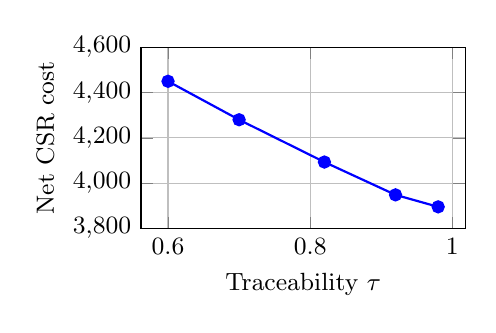
\begin{tikzpicture}
\begin{axis}[
    width=0.47\textwidth,
    height=0.32\textwidth,
    xlabel={Traceability $\tau$},
    ylabel={Net CSR cost},
    ymin=3800,
    ymax=4600,
    grid=major,
    tick label style={font=\small},
    label style={font=\small}
]
\addplot[blue, thick, mark=*] coordinates {
    (0.60,4450)
    (0.70,4280)
    (0.82,4093)
    (0.92,3948)
    (0.98,3895)
};
\end{axis}
\end{tikzpicture}
\hfill
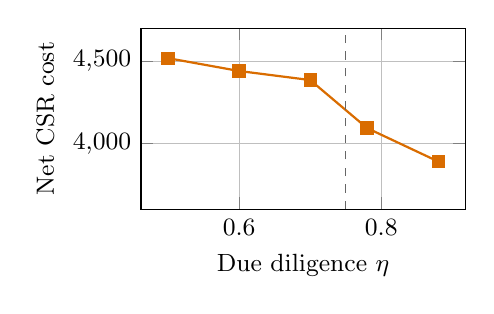
\begin{tikzpicture}
\begin{axis}[
    width=0.47\textwidth,
    height=0.32\textwidth,
    xlabel={Due diligence $\eta$},
    ylabel={Net CSR cost},
    ymin=3600,
    ymax=4700,
    grid=major,
    tick label style={font=\small},
    label style={font=\small}
]
\addplot[orange!85!black, thick, mark=square*] coordinates {
    (0.50,4518)
    (0.60,4440)
    (0.70,4385)
    (0.78,4093)
    (0.88,3890)
};
\addplot[black!60, dashed] coordinates {(0.75,3600) (0.75,4700)};
\end{axis}
\end{tikzpicture}
\caption{Traceability and Due-Diligence Sensitivity}
\label{fig:ch4_traceability_due_diligence}
\end{figure}

Figure~\ref{fig:ch4_traceability_due_diligence} visualizes two different mechanisms. The traceability curve is relatively smooth because higher $\tau$ gradually tightens the leakage bound and improves recovery information. The due-diligence curve has a visible threshold around the processor-access requirement. Once $\eta(S)$ crosses the high-standard processor threshold, the coalition can use a better recovery option, and the net cost drops more sharply. This is the graphical version of Proposition~\ref{prop:ch4_processor_threshold}.

\begin{figure}[htbp]
\centering
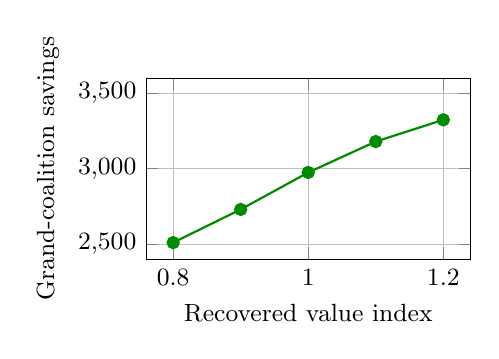
\begin{tikzpicture}
\begin{axis}[
    width=0.47\textwidth,
    height=0.32\textwidth,
    xlabel={Recovered value index},
    ylabel={Grand-coalition savings},
    ymin=2400,
    ymax=3600,
    grid=major,
    tick label style={font=\small},
    label style={font=\small}
]
\addplot[green!55!black, thick, mark=*] coordinates {
    (0.80,2510)
    (0.90,2730)
    (1.00,2975)
    (1.10,3180)
    (1.20,3324)
};
\end{axis}
\end{tikzpicture}
\hfill
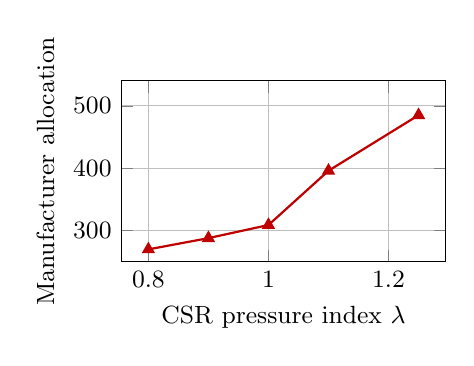
\begin{tikzpicture}
\begin{axis}[
    width=0.47\textwidth,
    height=0.32\textwidth,
    xlabel={CSR pressure index $\lambda$},
    ylabel={Manufacturer allocation},
    ymin=250,
    ymax=540,
    grid=major,
    tick label style={font=\small},
    label style={font=\small}
]
\addplot[red!75!black, thick, mark=triangle*] coordinates {
    (0.80,270)
    (0.90,288)
    (1.00,309)
    (1.10,396)
    (1.25,485)
};
\end{axis}
\end{tikzpicture}
\caption{Recovery-Value and CSR-Pressure Sensitivity}
\label{fig:ch4_recovery_pressure}
\end{figure}

Figure~\ref{fig:ch4_recovery_pressure} shows how financial and governance variables enter different parts of the model. Higher recovered-material value increases the savings game value $v(N)$ because the processor credit offsets stewardship cost. Higher CSR pressure raises the Manufacturer allocation because the Manufacturer's governance platform becomes more valuable for reducing risk and documenting compliance. The effect is nonlinear because the Shapley value averages marginal cost changes over coalitions, some of which benefit more from the Manufacturer's platform than others---the mechanism behind Proposition~\ref{prop:ch4_nonlinear_allocation}.

\begin{figure}[htbp]
\centering
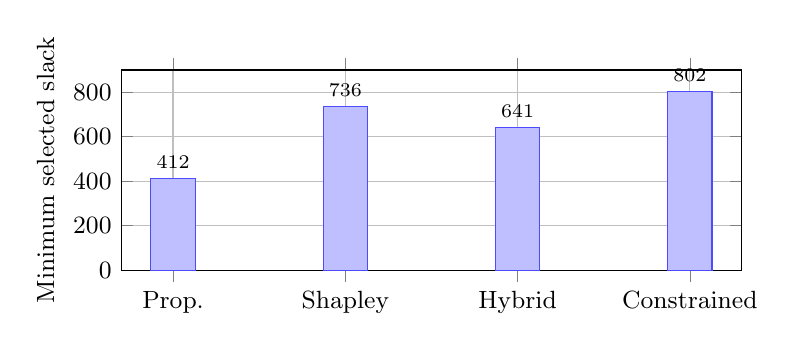
\begin{tikzpicture}
\begin{axis}[
    ybar,
    width=0.78\textwidth,
    height=0.34\textwidth,
    ylabel={Minimum selected slack},
    symbolic x coords={Prop., Shapley, Hybrid, Constrained},
    xtick=data,
    ymin=0,
    ymax=900,
    nodes near coords,
    nodes near coords style={font=\scriptsize},
    tick label style={font=\small},
    label style={font=\small},
    bar width=16pt,
    grid=major
]
\addplot[fill=blue!25, draw=blue!70] coordinates {
    (Prop.,412)
    (Shapley,736)
    (Hybrid,641)
    (Constrained,802)
};
\end{axis}
\end{tikzpicture}
\caption{Coalition-Stability Slack Under Alternative Allocation Rules}
\label{fig:ch4_allocation_slack}
\end{figure}

Figure~\ref{fig:ch4_allocation_slack} reinforces the Phase II logic. The proportional rule is easy to explain but produces the weakest selected stability margin in this stylized case. Shapley improves stability because it accounts for scale economies and governance contributions. The constrained projection performs best on the selected core checks because it explicitly optimizes closeness to Shapley subject to stability restrictions. The figure does not imply that one rule is always best; it shows how the model can diagnose allocation rules using the same coalition-cost function.

\subsection{Managerial and Policy Implications}

The case study yields three implications. First, CSR-oriented reverse logistics should not be treated as a pure logistics problem. Facility opening, routing, processor choice, compliance infrastructure, traceability, due diligence, and recovered-material value jointly determine the cost of credible CSR performance.

Second, volume-only cost sharing is incomplete. Retailers with high volume impose higher variable cost, but they also create scale economies. The Manufacturer may not contribute physical collection volume, but it can reduce cost through processor access, compliance routines, and recovery contracts. Shapley allocation is useful because it prices these marginal effects rather than assigning cost only by tons collected.

Third, fair allocation is a stability condition. If a retailer or the Manufacturer can do better outside the grand coalition, CSR cooperation is fragile. The core, individual-rationality, and stability-slack checks therefore serve as governance diagnostics. They identify whether the proposed CSR network can be supported by the allocation rule alone or whether additional contracts, constrained allocation, or Manufacturer support are needed.

% ============================================================
\section{Discussion: CSR Insights, Novelty, and Research Directions}
\label{sec:ch4_discussion}
% ============================================================

The preceding sections developed and illustrated the two-phase model. This section steps back from the derivations and asks what the model teaches about CSR governance, where its contribution sits relative to the surrounding literatures and frameworks, and which research directions it opens.

\subsection{What the Model Implies for CSR Governance}

Four governance insights emerge from the analysis, and none of them is visible in models that treat CSR as a scalar effort or preference.

First, \emph{CSR credibility is a capability problem before it is a preference problem}. Proposition~\ref{prop:ch4_feasibility} shows that a coalition cannot operate a compliant reverse network without sufficient physical capacity and sufficient due-diligence maturity to access certified processors. A firm can sincerely prefer responsible end-of-life treatment and still be unable to deliver it. This reframes the managerial question from ``how much does the firm care about CSR?'' to ``what combination of infrastructure, documentation, and contractual eligibility does credible CSR require, and who in the channel can supply each piece?''

Second, \emph{governance investment is conditionally, not automatically, valuable}. Proposition~\ref{prop:ch4_governance_value} gives the exact condition: traceability systems, audits, and compliance programs pay for themselves only when avoided leakage penalties, improved processor economics, better recovery value, and reduced coordination friction jointly exceed their cost. The model therefore resists both poles of the CSR debate---the claim that responsibility always pays and the claim that it is pure cost. Which pole is closer to the truth is a parameter question, and the model identifies which parameters decide it: CSR pressure $\lambda$, recovery-value responsiveness to documentation, and the processor-eligibility structure.

Third, \emph{capability thresholds make CSR economics discontinuous}. Because processor eligibility, facility openings, and capacity limits are discrete, small changes in due-diligence maturity or volume can produce large jumps in coalition cost and, through Proposition~\ref{prop:ch4_nonlinear_allocation}, in individual allocations. The practical consequence is that CSR governance investments should be planned against thresholds rather than average returns: an investment that moves a coalition just past a processor-eligibility threshold can be worth far more than its marginal cost suggests, while the same investment far from any threshold may show little effect. The due-diligence curve in Figure~\ref{fig:ch4_traceability_due_diligence} makes this visible.

Fourth, \emph{fair allocation is a stability condition, not a rhetorical flourish}. Efficiency guarantees that the CSR budget balances; it does not guarantee that anyone wants to stay in the coalition. The individual-rationality, core, and stability-slack checks convert ``is the allocation fair?'' into inequalities that can be verified against the actual coalition costs, and the least-core value $\epsilon^*$ and minimum subsidy $B^*$ quantify precisely how much contractual support is needed when the answer is no. In this framework, a Manufacturer subsidy is not philanthropy; it is the price of coalition stability, computable in advance.

\subsection{Novelty and Positioning}

The framework's contribution can be stated against three literatures. Relative to game-theoretic CSR channel models \cite{Buccella2024,FantiBuccella2017,Ferrara2017,Khosroshahi2019,Mahdiraji2023}, the model replaces the scalar CSR effort with a capability vector $G(S)=(\tau,\eta,\kappa)$ whose components have distinct operational consequences---leakage bounds, processor eligibility, and coordination cost. CSR is thereby modeled as something a coalition \emph{implements} rather than something a firm \emph{chooses a level of}. Relative to reverse-logistics network design \cite{tadaros2022location,bafadal2024proposed,wang2025planning,ma2024unlocking}, the model removes the implicit central planner: the optimized network must be financed by independent firms, and the financing question feeds back into whether the network is viable at all. Relative to cooperative allocation studies \cite{lozano2013cooperative,wang2023collaborative,meng2023profit,luo2022core}, the characteristic function is derived from the physical design problem rather than specified exogenously, so every stability check refers to a cost that a deviating coalition could actually realize.

The capability constructs also connect the model to the architecture of contemporary CSR governance frameworks, even though the chapter remains analytical. International guidance on social responsibility, such as ISO~26000, emphasizes stakeholder engagement, integration of responsibility into organizational processes, and communication of commitments and performance; sustainability-reporting frameworks such as the GRI standards center on impacts and embed human-rights and environmental due diligence; investor-facing disclosure standards such as IFRS~S1 and~S2 organize sustainability information around governance, strategy, risk management, and metrics; and the EU Corporate Sustainability Due Diligence Directive extends due-diligence obligations across value chains. In this language, the model's traceability parameter $\tau(S)$ is a metrics-and-transparency capability; the due-diligence parameter $\eta(S)$ is a value-chain due-diligence capability that gates access to certified partners; and the collaboration parameter $\kappa(S)$ is a governance-integration capability. The chapter thus offers a bridge, still rare in the modeling literature, between the constructs these frameworks describe qualitatively and the operational and allocative consequences a formal model can derive. The circular-economy motivation is equally grounded: recovering battery materials at scale is both an environmental obligation and a critical-mineral opportunity \cite{Harper2019}, and U.S. regulatory guidance already routes large-format batteries away from ordinary waste channels \cite{EPA2026UsedLithiumIon,EPA2026UniversalWaste}.

\subsection{Limitations and Research Directions}

The model's boundaries are deliberate, and each one defines a research direction.

First, the operational core is deterministic, linear in variable costs, and single-period, and coalition formation is one-shot. Real battery stewardship systems face uncertain return volumes, evolving chemistry mixes, volatile commodity prices, and repeated interaction among partners. Stochastic-programming or robust versions of Phase~I, and dynamic or repeated-game versions of Phase~II in which coalitions form, learn, and renegotiate over time, are natural extensions; system-dynamics or agent-based implementations could additionally capture informal-channel leakage and adoption dynamics that a static MILP cannot.

Second, the governance parameters $\tau$, $\eta$, and $\kappa$ are analytical primitives in this chapter, not measured constructs. A significant empirical agenda follows: operationalizing the three capabilities through survey instruments and archival disclosure coding, calibrating the MILP with observed regional volumes and facility costs, and testing whether measured governance capability predicts formal-channel capture and coalition cost as the model implies. A mixed-methods design---combining survey-based constructs, disclosure data, model-generated coalition costs, and interviews with stewardship managers---would allow the stylized case of Section~\ref{sec:case_study} to be replaced by a validated application, and would connect the model to the measurement traditions of the empirical CSR literature.

Third, fairness in this chapter is economic: an allocation is acceptable when it beats outside options. Behavioral research on cost sharing suggests that acceptance also depends on procedural fairness---transparency of the rule, opportunity for voice, consistency of application---and on power asymmetry among partners. Whether coalition members accept a Shapley-based rule they cannot easily verify, and whether the hybrid rule's responsibility weights $p_x$ improve perceived legitimacy even when they worsen stability slack, are open behavioral questions that vignette experiments or negotiation studies could address. The remedies of Section~\ref{sec:game_theory} give such studies a precise set of treatments to compare.

Fourth, the case study is illustrative, and the chapter's numerical claims are claims about the model, not about the U.S. industry. A reproducible solver implementation with calibrated data---regional return-volume estimates, facility cost benchmarks, and observed processor economics---is the most direct next step and would also enable the full-enumeration Shapley and least-core computations for larger retailer sets.

These directions share a theme: the two-phase structure developed here is designed to be a stable core. Uncertainty enters through Phase~I parameters, behavior enters through Phase~II acceptance, and measurement enters through the capability vector. The framework is therefore extensible without being rebuilt.

% ============================================================
\section{Conclusion}
\label{sec:model_conclusion}
% ============================================================

This chapter developed Study~2 of the dissertation: a CSR-based multi-retailer reverse-logistics model with Shapley cost sharing. Extending the bilateral CSR coordination logic of Chapter~\ref{chap:model1} to a network setting, the model asks how a shared CSR infrastructure should be designed and how its cost should be allocated. Phase~I formulates a coalition-dependent MILP for net CSR stewardship cost, in which traceability, due diligence, and collaborative governance shape leakage, processor eligibility, recovery value, and coordination cost. Phase~II uses the optimized coalition costs as a cooperative cost game and applies the Shapley value.

The central analytical message is the division of labor between what allocation theory guarantees and what the application must verify. Shapley allocation always funds the network, but participation and coalition stability depend on the coalition-cost function the physical model generates; they must be checked, not asserted. When the checks fail, the chapter provides mathematically explicit remedies---hybrid responsibility allocation, constrained Shapley projection, least-core diagnostics, and Manufacturer support---each of which converts a fairness problem into a computable governance instrument.

The stylized U.S. EV battery recycling case illustrated the full workflow: the grand coalition reduced net stewardship cost by roughly forty percent relative to stand-alone operation, the Shapley allocation passed the reported participation and stability checks, and the sensitivity analysis traced how governance capability, recovery value, and CSR pressure move both network design and cost allocation. More broadly, the chapter shows that CSR in reverse logistics is a governance problem: responsible collection and processing require both an efficient physical network and a cost-sharing rule that independent stakeholders can accept. Section~\ref{sec:ch4_discussion} sets out how this framework can be calibrated, stressed, and behaviorally validated in subsequent research.
